\chapter{Metodología}\label{chapter:proposal}
En este capítulo se exponen los diferentes procedimientos y métodos empleados durante el estudio. Primeramente, se explica el procesamiento y manejo de los datos. Se exponen además análisis exploratorios iniciales de los datos que repercuten en las decisiones de implementación. Por último se describen los métodos utilizados para el cálculo de la variable decisora en el estudio de inmunopuente y se especifican las herramientas computacionales utilizadas.

\section {Fuentes de datos utilizadas}

Para el desarrollo de este trabajo se tuvieron en cuenta los resultados correspondientes a dos ensayos clínicos:
\begin{itemize}
	\item Ensayo clínico fase II/III, multicéntrico, aleatorizado, doble ciego, de grupos paralelos secuenciales; con el objetivo de evaluar la inmunogenicidad y eficacia de Quimi-Vio 7 contra neumococos en niños pre-escolares. Se incluyeron un total de 1132 sujetos de 1140 enrolados, con una distribución de 570 sujetos en  la  primera etapa y 562 en la segunda. De ellos, se  midió la actividad opsonofagocítica de 67 participantes ($n = 67$).
	
	El ensayo reportó una eficacia protectora global de 94.4\% para Quimi-Vio 7 frente al 96.38\% de PREVNAR13\textsuperscript{\textregistered}, para sus cinco serotipos comunes, demostrando no inferioridad respecto a la vacuna de referencia internacional y sustentando  su empleo como vacuna de referencia en el presente estudio. Además las tasas de seroconversión fueron superiores al 80\% para todos los serotipos tanto en el grupo de estudio como en el grupo de control. 
	
	
	\item Ensayo clínico fase II/III, de combinación de etapas, controlado, aleatorizado, doble ciego en la fase II,  de no inferioridad, adaptativo y multicéntrico, para evaluar la inmunogenicidad, seguridad y eficacia del candidato vacunal conjugado 11-valente Quimi-Vio 11 contra neumococos en adultos entre 50 y 74 años. Con un total de 1001 participantes y medición de títulos opsonofagocíticos de $n = 65$ individuos. El objetivo central de este ensayo fue evaluar la no inferioridad inmunológica de Quimi-Vio 11 respecto a  PREVNAR13\textsuperscript{\textregistered}.
\end{itemize}

La variable inmunológica de ambos ensayos que se empleó en este estudio fueron los títulos opsonofagocíticos registrados un mes después de la vacunación.

El ensayo clínico de Quimi-Vio 7 incluyó mediciones para nueve serotipos: los siete contenidos en la formulación vacunal (1, 5, 14, 6B, 18C, 19F y 23F) y dos serotipos relacionados de relevancia clínica (6A y 19A) para los que también se registró respuesta inmunológica. Quimi-Vio 11 registró estos mismos serotipos y adicionalmente los serotipos 9V y 22F, para un total de once.

El análisis de inmunopuente se realizó sobre los nueve serotipos comunes a ambos ensayos. Los datos fueron suministrados en formato Excel y PDF, y sometidos a un proceso de extracción, limpieza y transformación.

\subsection{Procesamiento y manejo de datos inmunológicos}

El pipeline de procesamiento de los datos se estructuró en cuatro fases consecutivas, que abarcan desde la recopilación de los datos procedentes de los ensayos clínicos hasta la obtención de los conjuntos de datos finales empleados en el análisis estadístico y la modelación. La Figura~\ref{fig:data_cycle} resume las etapas que conforman este flujo de trabajo.

\begin{figure}[ht]
	\centering
	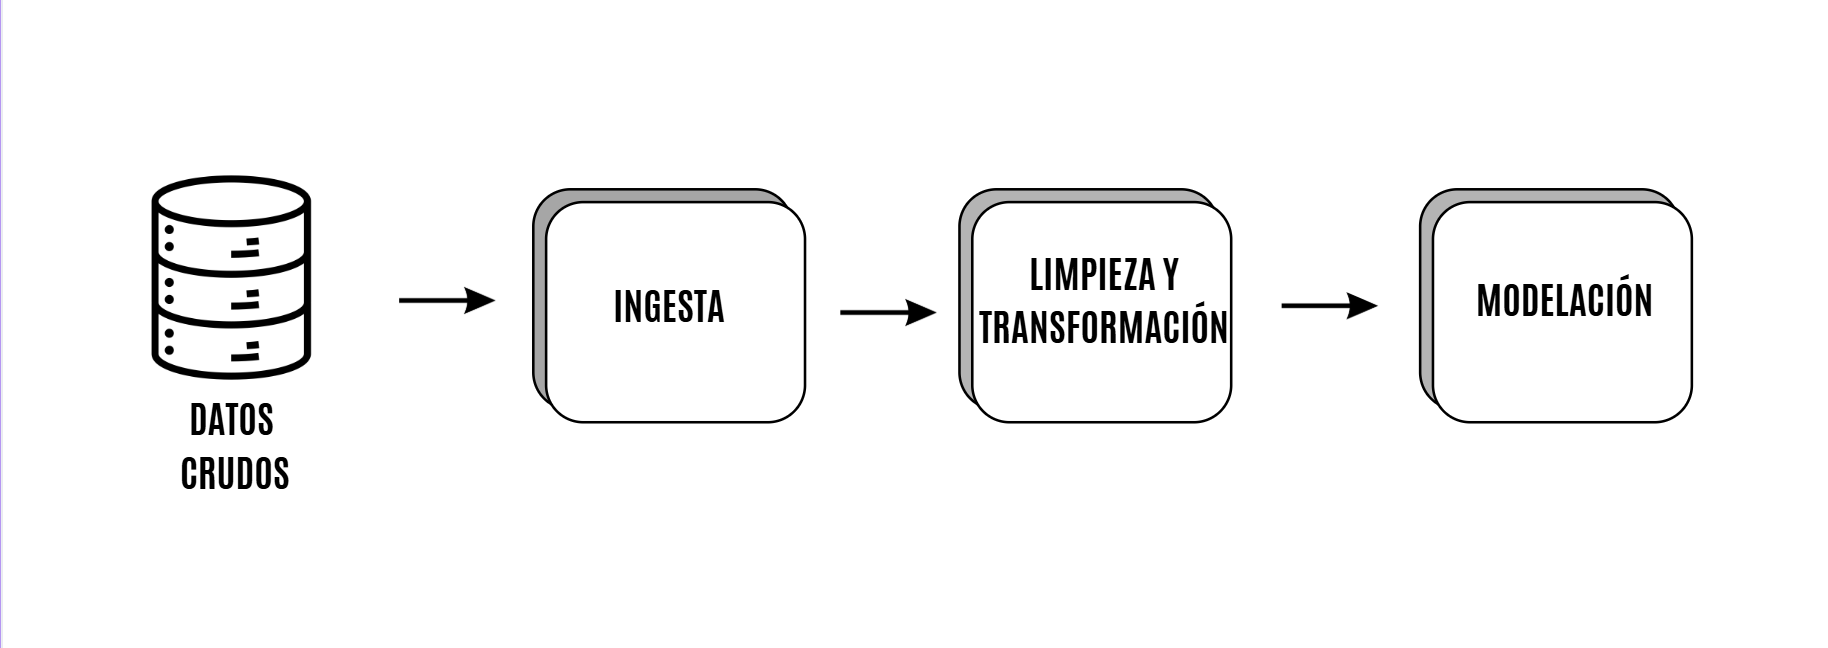
\includegraphics[width=0.9\textwidth]{Graphics/esquema.png}
	\caption{Etapas del tratamiento de los datos de inmunogenicidad durante el estudio.}
	\label{fig:data_cycle}
\end{figure}
\FloatBarrier

A continuación se explican cada una de las fases del pipeline de forma más detallada.

\subsection{Ingesta y extracción}

El proceso de extracción se realizó a partir de los registros originales de ambos ensayos clínicos y se almacenaron en archivos en formato \texttt{.csv} para garantizar su correcta integración y una estructura estandarizada que facilitara su posterior análisis y procesamiento.

\subsection{Limpieza}

Una vez almacenados los datos, se identificaron los registros con valores faltantes en los títulos de anticuerpos por serotipo. Debido a que la proporción de datos ausentes no superó el 6.3\% en ninguno de los serotipos analizados, se decidió eliminar dichas observaciones antes de continuar con el análisis, al considerarse que este nivel de pérdida no compromete la representatividad de la muestra ni la validez de las inferencias posteriores.

\begin{table}[ht]
	\centering
	\caption{Cantidad de valores faltantes por serotipo en los datos de OPA.}
	\label{tab:nulls_opa}
	\small
	\begin{tabular}{lccccccccccc}
		\hline
		& Sp1 & Sp5 & Sp6A & Sp6B & Sp9V & Sp14 & Sp18C & Sp19A & Sp19F & Sp23F & Total \\
		\hline
		Niños   & 0 & 0 & 0 & 0 & 0 & 0 & 0 & 0 & 0 & 0 & 0  \\
		Adultos & 2 & 2 & 2 & 1 & 9 & 1 & 3 & 2 & 4 & 1 & 27 \\
		\hline
		Total   & 2 & 2 & 2 & 1 & 9 & 1 & 3 &2 & 4 & 1 & 27 \\
		\hline
	\end{tabular}
\end{table}
\FloatBarrier

Se eliminaron, además, valores inconsistentes como por ejemplo valores negativos.

\begin{table}[ht]
	\centering
	\caption{Tamaño muestral final por serotipo después del preprocesamiento.}
	\label{tab:n_final_serotipos}
	\begin{tabular}{lccccccccc}
		\hline
		& Sp1 & Sp5 & Sp6A & Sp6B & Sp14 & Sp18C & Sp19A & Sp19F & Sp23F \\
		\hline
		Niños   & 81 & 80 & 75 & 81 & 82 & 78 & 81 & 82 & 83 \\
		Adultos & 63 & 63 & 63 & 64 & 64 & 62 & 63 & 61 & 64 \\
		\hline
	\end{tabular}
\end{table}

\FloatBarrier

\subsection{Transformación}

Cuando se trabaja con datos de inmunogenicidad se asume log-normalidad de los datos \cite{nauta2020}, es por eso que luego de la limpieza de los mismos, se transformaron a escala logarítmica.
\begin{figure}[ht]
	\centering
	
	\begin{subfigure}{0.4\textwidth}
		\centering
		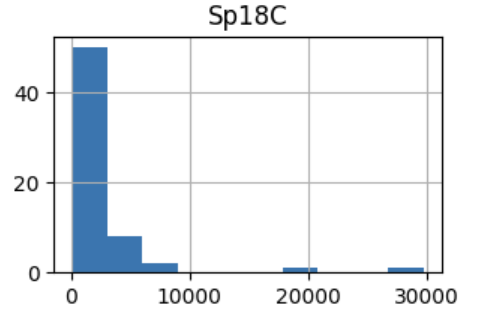
\includegraphics[width=\linewidth]{Graphics/adultos18cantes.png}
		\caption{Antes}
	\end{subfigure}
	\hfill
	\begin{subfigure}{0.4\textwidth}
		\centering
		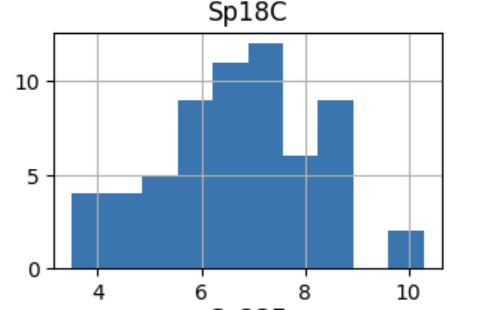
\includegraphics[width=\linewidth]{Graphics/adultos18cdespues.png}
		\caption{Después}
	\end{subfigure}
	
	\caption{Serotipo 18C en adultos antes y después de transformación logarítmica.}
	\label{fig:comparacion 18C}
\end{figure}

\begin{figure}[ht]
	\centering
	
	\begin{subfigure}{0.45\textwidth}
		\centering
		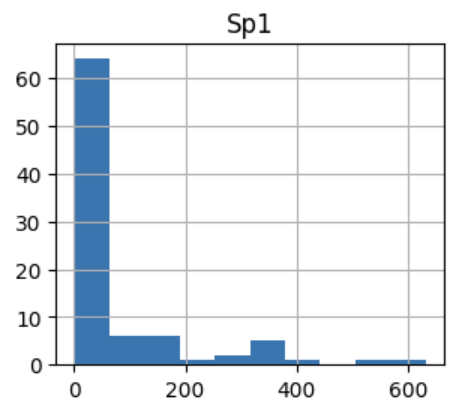
\includegraphics[width=\linewidth]{Graphics/ninnos1antes.png}
		\caption{Antes}
	\end{subfigure}
	\hfill
	\begin{subfigure}{0.45\textwidth}
		\centering
		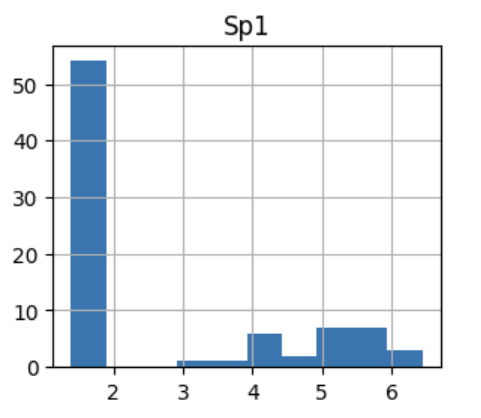
\includegraphics[width=\linewidth]{Graphics/ninnos1despues.png}
		\caption{Después}
	\end{subfigure}
	
	\caption{Serotipo 1 en niños antes y después de transformación logarítmica.}
	\label{fig:comparacion 1}
\end{figure}

\FloatBarrier

\subsection{Valores por debajo del límite inferior de cuantificación (LLOQ)}

Los datos correspondientes a respuestas opsonofagocíticas por debajo del LLOQ se trataron como datos censurados por la izquierda. Siguiendo la práctica estándar en la literatura inmunológica, estos valores fueron imputados con el valor fijo de $LLOQ/2$ \cite{Essink2022, Solanki2017}. Sin embargo, para evitar estimaciones sesgadas, se analizó la magnitud de este fenómeno en la muestra.

En las figuras \ref{fig:LLOQ_niños} y \ref{fig:LLOQ_adultos} se muestra el porcentaje real de valores censurados obtenidos en las poblaciones de niños y adultos.

\begin{figure}[ht]
	\centering
	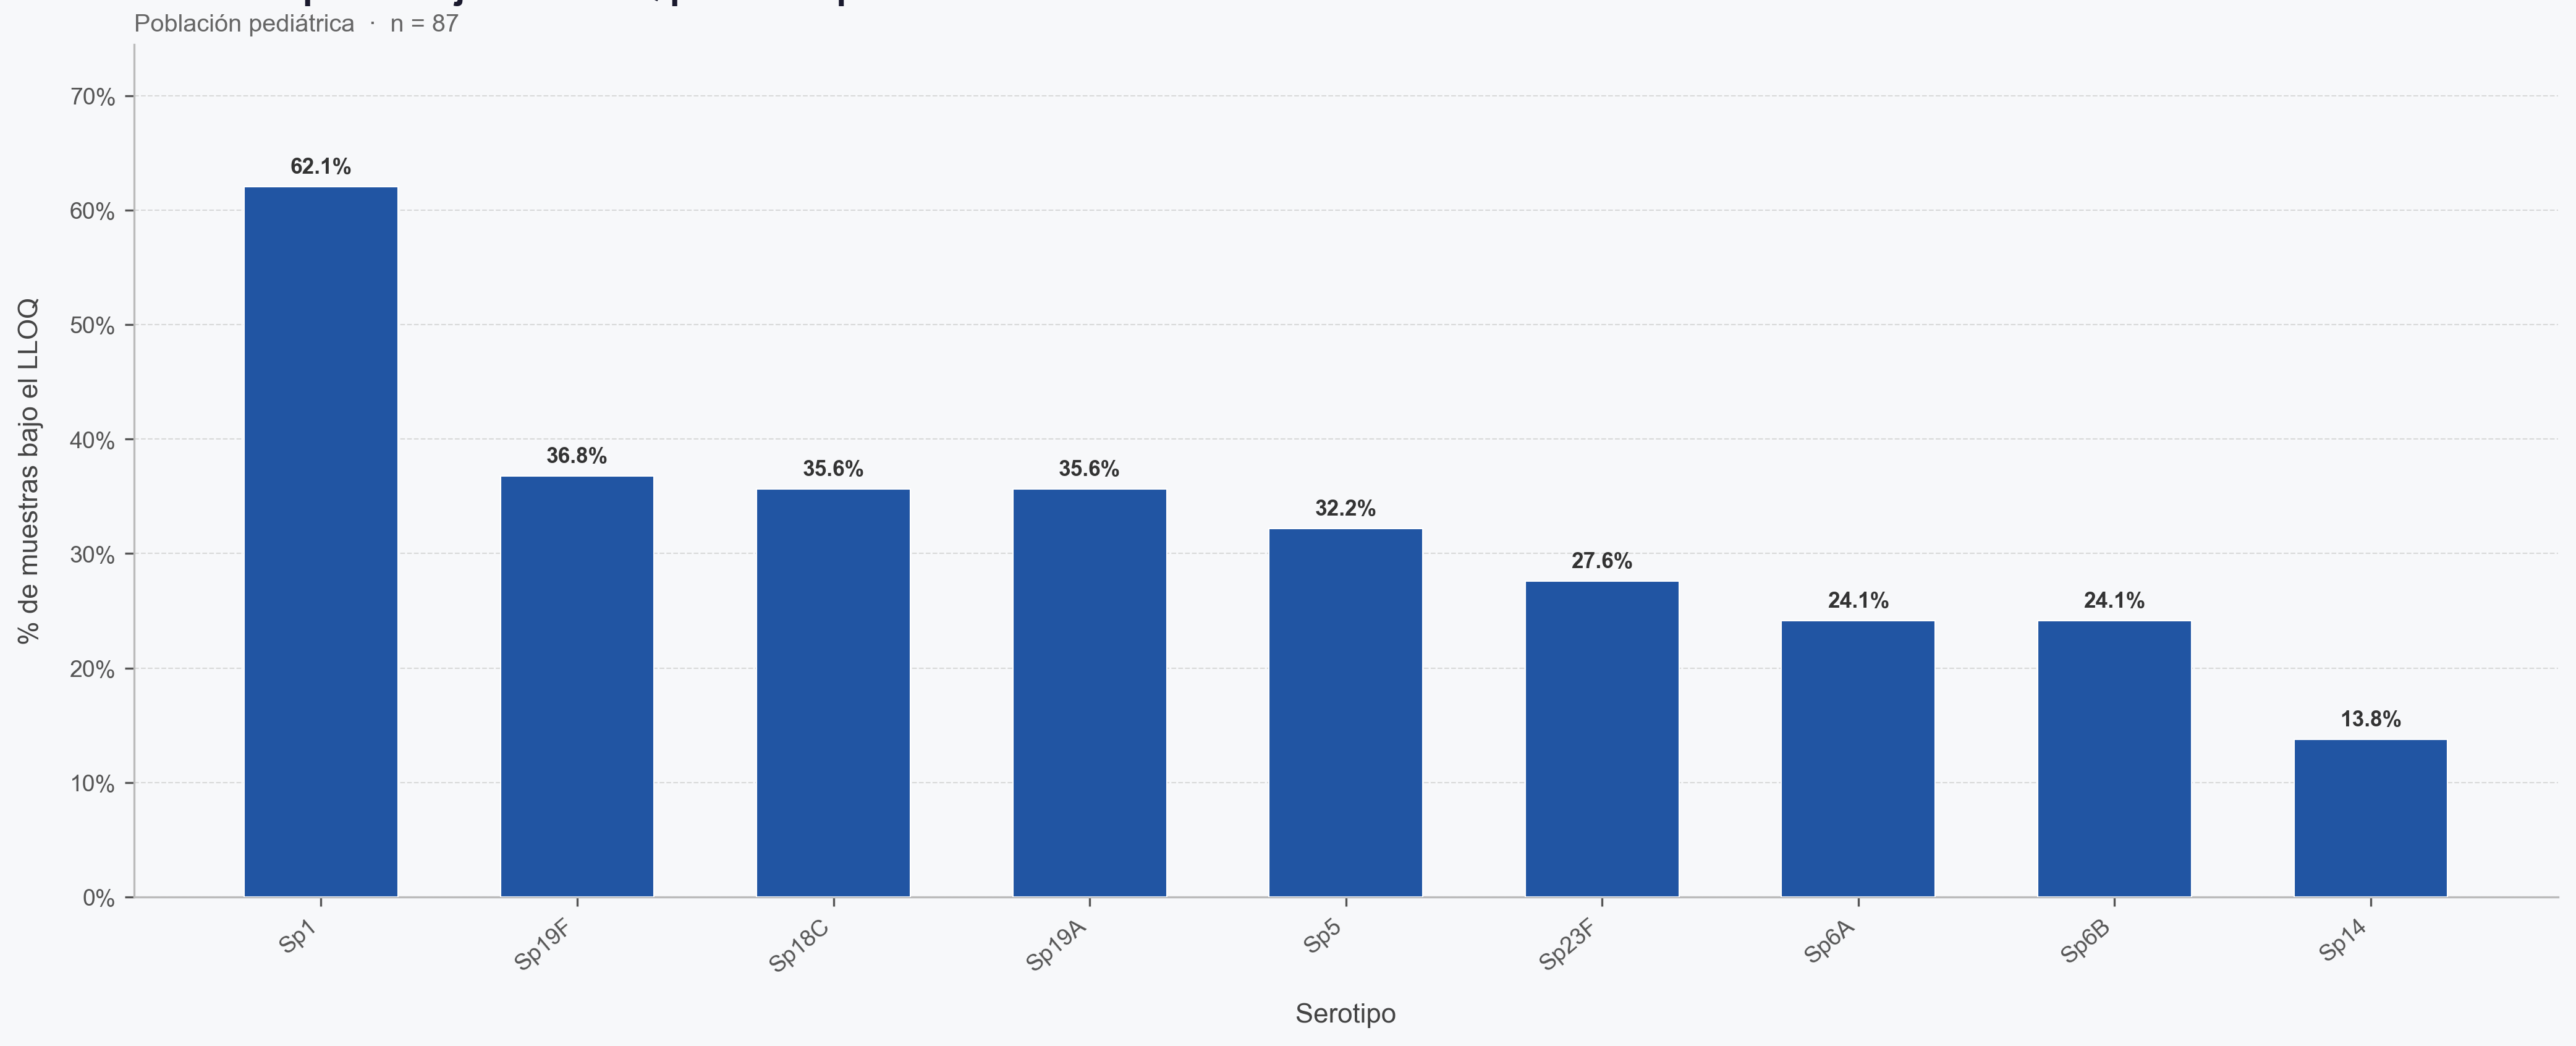
\includegraphics[width=0.9\textwidth]{Graphics/LLOQninnos.png}
	\caption{Porcentaje de registros por debajo del LLOQ en niños}
	\label{fig:LLOQ_niños}
\end{figure}

\FloatBarrier

\begin{figure}[ht]
	\centering
	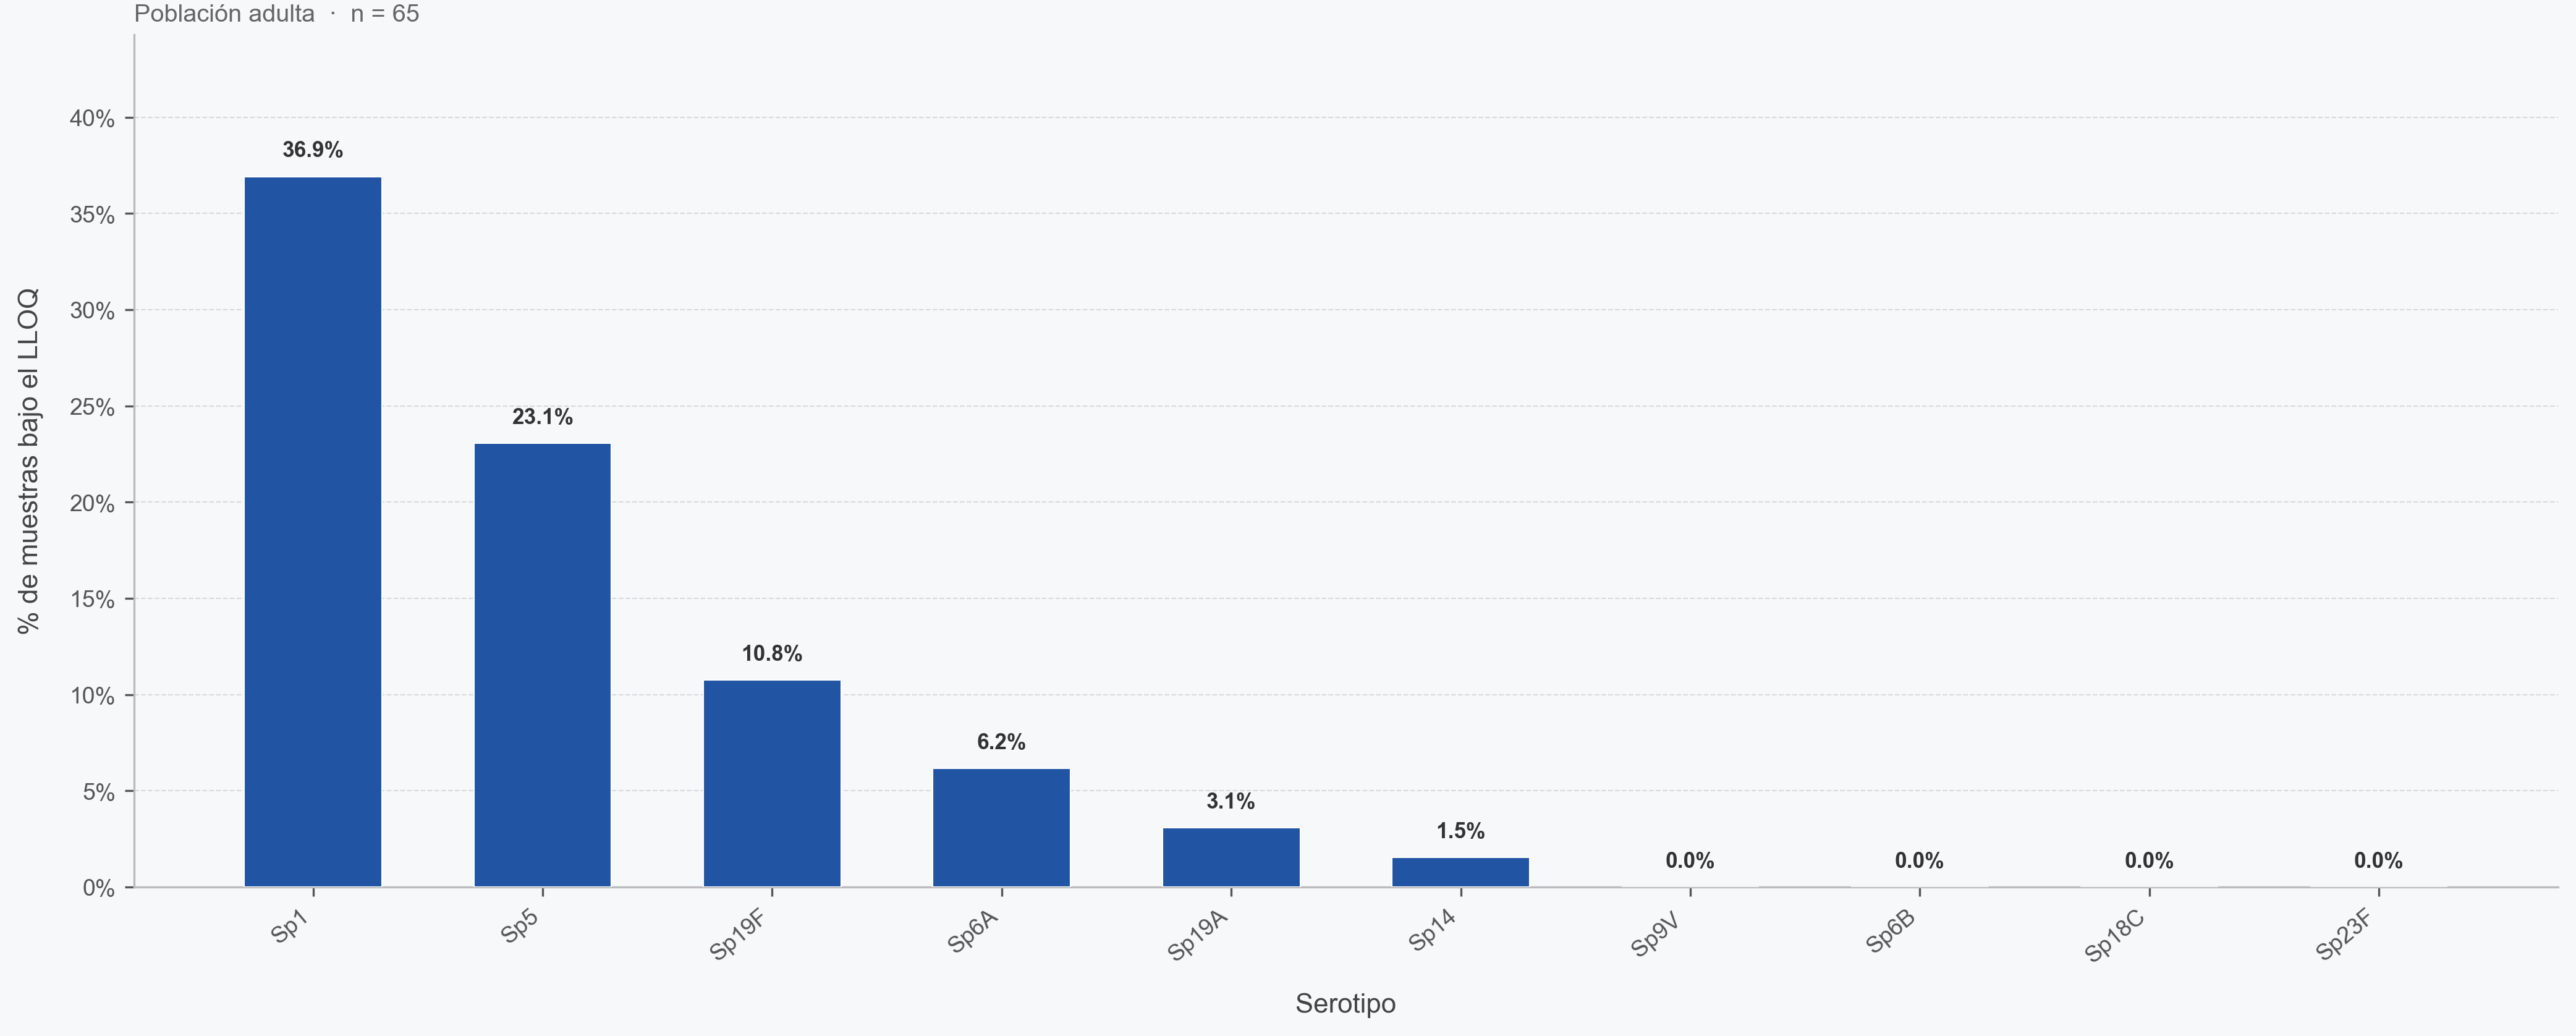
\includegraphics[width=0.9\textwidth]{Graphics/LLOQadultos.png}
	\caption{Porcentaje de registros por debajo del LLOQ en adultos}
	\label{fig:LLOQ_adultos}
\end{figure}

\FloatBarrier

Como se observa, tanto en niños como en adultos se presentaron serotipos con niveles de censura superiores al 30\%. Por lo tanto, para el análisis estadístico posterior (sección \ref{sec:Métodos_de_estimación_utilizados}) además de los análisis tradicionales, se optó por el uso de un modelo de máxima verosimilitud, capaz de mitigar el sesgo inducido por este alto volumen de censura.

\section{Modelación}

La evaluación de la respuesta inmunológica se determinó a partir de la Medias Geométricas de los Títulos (GMT) y la Razón de Medias Geométricas (GMR).

Las GMT se calcularon de manera independiente para cada uno de los serotipos. Luego la GMR se define específicamente como la razón entre la media geométrica en adultos (grupo de prueba) y la media geométrica de niños (grupo de referencia) para cada serotipo, es decir:

\[
\mathrm{GMR} = \frac{\mathrm{GMT}_{\mathrm{adultos}}}
{\mathrm{GMT}_{\mathrm{ni\tilde{n}os}}}
\]

Esta variable se utilizó como métrica principal para el inmunopuente y se demuestra no inferioridad del serotipo si:

\[
\mathrm{LI}_{95\%}\!\left(\mathrm{GMR}\right) > 0.5
\]

Es decir, si el límite inferior del intervalo de confianza bilateral al 95\% de la razón de medias geométricas es mayor que 0.5, como estándar regulatorio empleado en estudios similares \cite{platt2024safety, Essink2022, mcelwee2026overview, jacksonnew}.

\subsection{Métodos de estimación utilizados}\label{sec:Métodos_de_estimación_utilizados}

Teniendo en cuenta el alto porcentaje de censura en los datos para muchos de los serotipos involucrados, se emplearon dos métodos para la estimación de los valores referentes a las medias geométricas de los títulos de anticuerpo: el \textbf{método de sustitución simple} y el \textbf{método de estimación por máxima verosimilitud}. A continuación se explica a detalle cómo se emplearon ambos métodos.

\begin{itemize}
	\item \textbf{Sustitución}\\
	En este método se conservó la imputación inicial que se empleó en la base de datos para introducir todos los valores por debajo del límite inferior de cuantificación, por lo que el cálculo de la media geométrica en este caso coincide con la exponencial de la media aritmética de los logaritmos, como aparece en \ref{eq:gmt_2}.
	
	Luego los intervalos de confianza se calcularon mediante la aproximación de Welch para $\alpha = 0.05$, puesto que no se cumple la homocedasticidad entre ambas muestras.
	
	\begin{table}[ht]
		\centering
		\caption{Prueba de Levene para homogeneidad de varianzas por serotipo}
		\label{tab:levene}
		\begin{tabular}{lccc}
			\toprule
			Serotipo & Estadístico Levene & p-valor & Homocedasticidad \\
			\midrule
			Sp1   & 9.2248  & 0.0028 & No \\
			Sp5   & 0.0623  & 0.8032 & Sí \\
			Sp6A  & 10.4530 & 0.0015 & No \\
			Sp6B  & 5.7094  & 0.0182 & No \\
			Sp14  & 10.0163 & 0.0019 & No \\
			Sp18C & 36.0272 & 0.0000 & No \\
			Sp19A & 24.0372 & 0.0000 & No \\
			Sp19F & 18.0979 & 0.0000 & No \\
			Sp23F & 15.9956 & 0.0001 & No \\
			\bottomrule
		\end{tabular}
	\end{table}
	
	\FloatBarrier
	
	\item \textbf{Estimación por Máxima Verosimilitud}\\
	
	Para corregir el sesgo inducido por la imputación de valores, se implementó un modelo de regresión lineal censurado por la izquierda (Modelo de Tobit) detallado en \ref{sec:Modelo_Tobit}.
	
	Los intervalos de confianza del 95\% para las GMT y las GMR estimadas por este método se calcularon mediante aproximaciones asintóticas de Wald.
	
	No obstante, dado que la validez de esta aproximación asintótica depende de que la función de verosimilitud sea aproximadamente cuadrática alrededor del estimador de máxima verosimilitud, una condición que puede no cumplirse en presencia de una alta proporción de datos censurados y muestras de tamaño moderado \cite{pawitan2001all}, se calcularon adicionalmente intervalos de confianza utilizando el perfil de verosimilitud \cite{venzon1988method} para verificar la adecuación de la aproximación de Wald en este caso.
	
\end{itemize}

\section{Detalles de implementación}

Todas las implementaciones necesarias para el procesamiento y análisis estadístico se realizaron en Python 3.12.8, utilizando las siguientes bibliotecas:

\begin{itemize}
	\item \texttt{Pandas}: Se empleó en el proceso de integración, limpieza de datos faltantes y estructuración de las tablas finales en formato CSV.
	\item \texttt{NumPy}: Se utilizó para la conversión de los títulos opsonofagocíticos a escala logarítmica y el cálculo de las medias geométricas tradicionales.
	\item \texttt{SciPy}: Se utilizó para la modelación avanzada mediante el Modelo Tobit, permitiendo la estimación de los valores de GMT por máxima verosimilitud y el cálculo de sus intervalos de confianza asintóticos.
	\item \texttt{Camelot}: Se utilizó para la extracción automatizada de las tablas de inmunogenicidad desde los reportes clínicos en formato PDF.
	\item \texttt{Matplotlib}: Se empleó en el diseño de las visualizaciones de los resultados y en el análisis exploratorio de los datos.
\end{itemize}

A continuación se exponen los resultados derivados de la aplicación de este enfoque metodológico.
